\documentclass{article}[12pt]

\usepackage{amsthm}
\usepackage{amssymb}
\usepackage{amsmath}
\usepackage{mathtools}

%\usepackage{fontspec}
\usepackage[margin=1in]{geometry}
\setlength{\parindent}{0pt}

\usepackage{indentfirst}
\usepackage{setspace}
\usepackage{graphicx}
\usepackage{wrapfig}
\usepackage{caption}
\usepackage{subcaption}
\usepackage{siunitx}
\usepackage{fancyhdr}
\usepackage{titlesec}


\theoremstyle{definition}
\newtheorem{theorem}{Theorem}
\newtheorem*{definition}{Definition}
\newtheorem*{example}{Example}
\newtheorem*{theorem*}{Theorem}

\newcommand{\myabs}[1]{\vert#1\vert}
\newcommand{\pder}[2]{\frac{\partial#1}{\partial#2}}
\newcommand{\pdder}[2]{\frac{\partial^2#1}{\partial#2^2}}
\newcommand{\dder}[2]{\frac{d^2#1}{d^2#2}}
\newcommand{\orb}{\mathcal{O}}

\DeclareMathOperator{\iso}{Iso}
\DeclareMathOperator{\fix}{Fix}
\DeclareMathOperator{\tr}{Tr}
\DeclareMathOperator{\vol}{vol}
\DeclareMathOperator{\divergence}{div}
\DeclareMathOperator{\grad}{grad}


\titleformat*{\section}{\Large\bfseries}

\pagestyle{fancy}
\fancyhf{}
\rhead{Sean Richardson}
\lhead{Lewis \& Clark Department of Mathematical Sciences}

\begin{document}
\singlespacing
\title{Hearing the Local Orientability of Orbifolds}
\author{Sean Richardson with research mentor Liz Stanhope}
\date{}
\maketitle
\thispagestyle{fancy}

\section{Background}

An orbifold is a generalization of a
\emph{manifold}, some $n$ dimensional surface. Recall a manifold is
defined through an atlas of compatible charts such that each chart maps
$\widetilde{U} \subset \mathbb{R}^n$ onto some subset of the manifold.
Note that each $\widetilde{U}$ must be open and connected.
The definition of an orbifold follows similarly.

\begin{definition}[Orbifold]
    For some orbifold $\mathcal{O}$ we take a group of isometries
    $\Gamma$ and some subset $\widetilde{U} \subset \mathbb{R}^n$. Then, we
    have some mapping $\pi_u$ the corresponding topological quotient
    $\widetilde{U}/\Gamma$ onto some subset $U \subset \mathcal{O}$. The
    tuple $(\widetilde{U},\Gamma,\pi_U)$ is called a \emph{chart}, and
    $\mathcal{O}$ is a valid orbifold if it has an atlas of compatible
    charts.
\end{definition}

We can then provide an orbifold with a Riemannian metric by patching
together Riemannian metrics on the local charts such that each metric is
invariant under the group action of each chart. In this paper, all
referenced orbifolds have an implied Riemannian metric.

\begin{definition}[Strata]
This construction gives rise to a natural partitioning of some orbifold
$\orb$ into a collection of submanifolds such that: each submanifold $N$ is
connected, and each point in $N$ has local structure with exactly the same
isometry group. We denote this group $\iso(N)$ and we call each such submanifold a \emph{strata} of $\orb$.
\end{definition}

There is a subclass of strata called \emph{primary singular strata} or
simple \emph{primary strata}. For the purposes of the paper, a strata $N$
is a \emph{primary strata} or simply \emph{primary strata} if
there exists some isometry $\gamma \in \iso(N)$ such that
$\dim(\fix(\gamma)) = \dim(N)$. Note that the $\fix$ operator denotes the
set of points where each point is mapped to itself under the isometry.

\begin{example}
    Take the group of isometries $G = \{\mathbb{Z} \times \mathbb{Z}, e,
    r_x,  r_y, R_{180}\}$. Here, $\mathbb{Z} \times \mathbb{Z}$ denotes the
    translation lattice by integers, $e$ denotes the identity, $r_x$ and
    $r_y$ are reflections across the $x$ and $y$ axes respectively, and
    $R_{180}$ denotes a rotation by $\ang{180}$. Note that without the
    translation lattice, this is the dihedral group $D_2$.  Now, we
    consider the topological quotient $\mathbb{R}^2/G$. This topological
    quotient forms a valid orbifold $\orb$. Orbifold $\orb$ has fundamental
    domain of a square with side lengths $\frac{1}{2}$; $\orb$ has $4$
    strata of dimension $1$ (mirror edges); and $\orb$ has $4$ strata of
    dimension $0$ (corner reflector). Each mirror edge has chart with
    isotropy group $\Gamma = \{e,r_x\}$ or $\Gamma = \{e,r_y\}$, and each
    corner reflector has the full dihedral group $\Gamma =
    \{e,r_x,r_y,R_{180}\}$. In the case of the mirror edges, $\fix(r_x)$
    and $\fix(r_y)$ is of dimension $1$, the same dimension as the strata
    making each mirror edge a primary strata. Similarly, $\fix(R_{180})$ is
    of dimension $0$, the same dimension of the corner reflectors, so each
    corner reflector is a primary strata. See `Asymptotic Expansion
    of the Heat Kernel for Orbifolds' 2.15 for more detail\cite{DGGW}.
\end{example}

%\indent In order to formally define orbifolds, we touch on symmetry groups. A
%symmetry group is a collection of actions, typically denoted $\Gamma$, we
%can perform on a pattern without change. For instance, we can rotate
%Figure~\ref{fig:rot_sym} by \ang{90}, \ang{180}, \ang{270}, or \ang{0} and
%still preserve the pattern. Similarly, Figure~\ref{fig:ref_sym} is
%preserved by the action of reflecting along the diagonal and doing nothing.
%
%Some actions are \emph{orientation preserving} such as rotations. A
%rotation would take a ``b'' to a ``b''. Conversely, some actions are
%orientation reversing such as reflections. These would take a ``b'' to a
%``d''.

%Note that in the patterns below, certain points (such as those marked by
%green dots) can be mapped to one another using the elements of the
%corresponding group. Then, if we define all such groups of points to be the
%same point, we obtain the \emph{quotient space}. We can visually represent
%this quotient space by overlapping the groups of paired points. In the case
%of rotational symmetry, we can twist the pattern into a party hat as shown
%in Figure~\ref{fig:cp} and for the reflectional symmetry, we fold across
%the diagonal as shown in Figure~\ref{fig:me}

%Next, note that there exist some points that are mapped to themselves for
%every element of the group. We call these collections of points
%\emph{strata}. In the patterns below, the blue center in
%Figure~\ref{fig:rot_sym} is a strata of dimension $0$, and the red diagonal
%in Figure~\ref{fig:ref_sym} is a strata of dimension $1$.

% \begin{figure}[h]
%     \centering
%        \begin{subfigure}{0.25\textwidth}
%        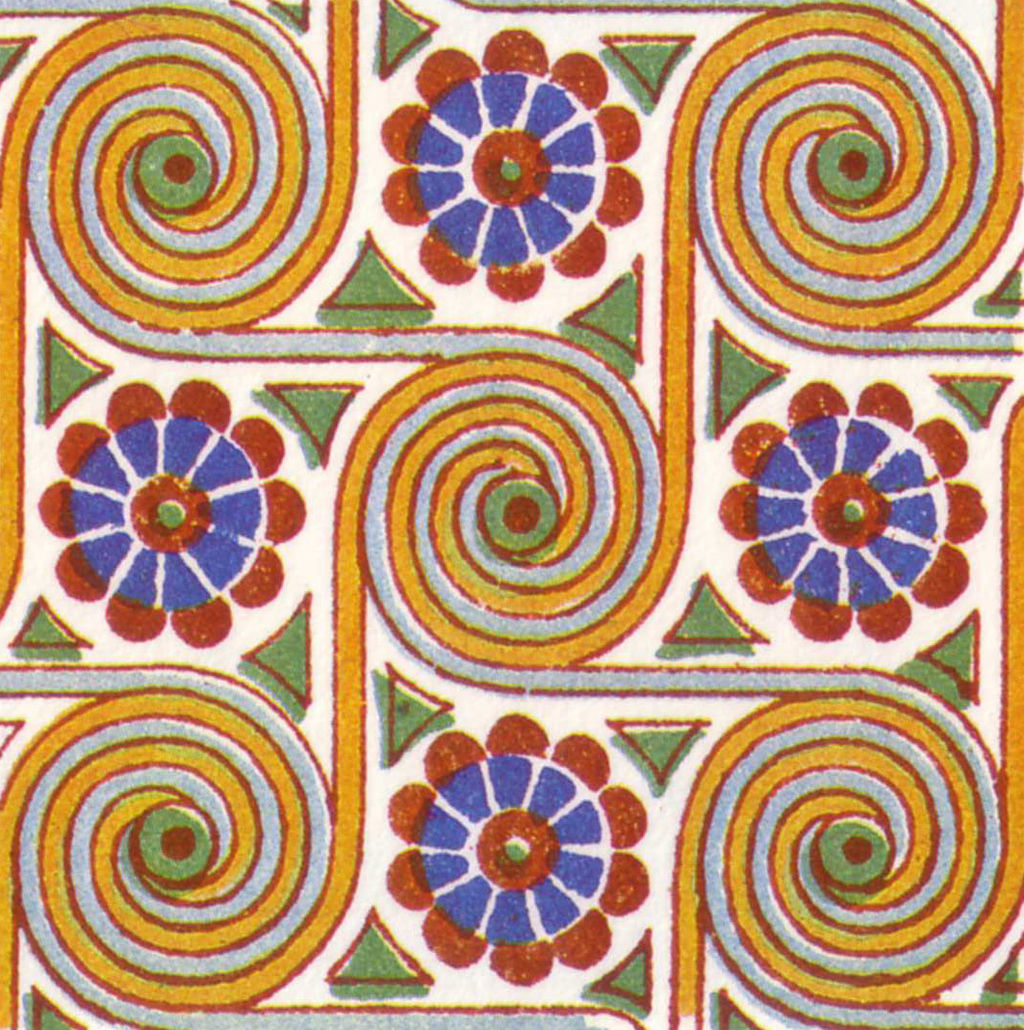
\includegraphics[width=\textwidth]{images/p4_symmetry_wallpaper.jpg}
%        \caption{Rotational Symmetry}
%        \label{fig:rot_sym}
%        \end{subfigure}
%        \begin{subfigure}{0.2\textwidth}
%            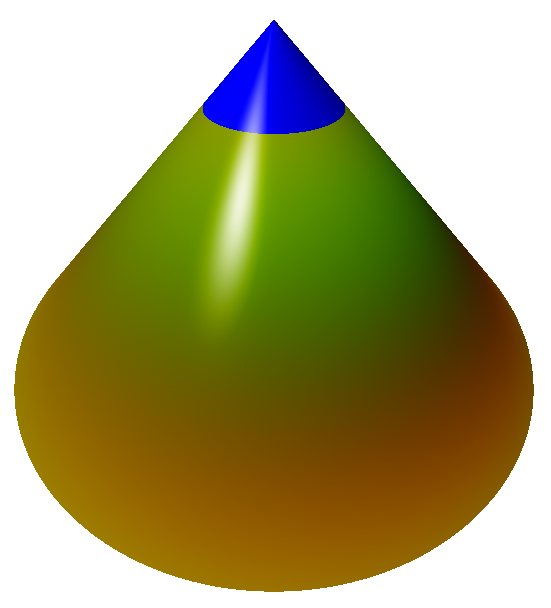
\includegraphics[width=\textwidth]{images/cone_point.png}
%            \caption{Cone Point}
%            \label{fig:cp}
%        \end{subfigure}
%        \begin{subfigure}{0.25\textwidth}
%        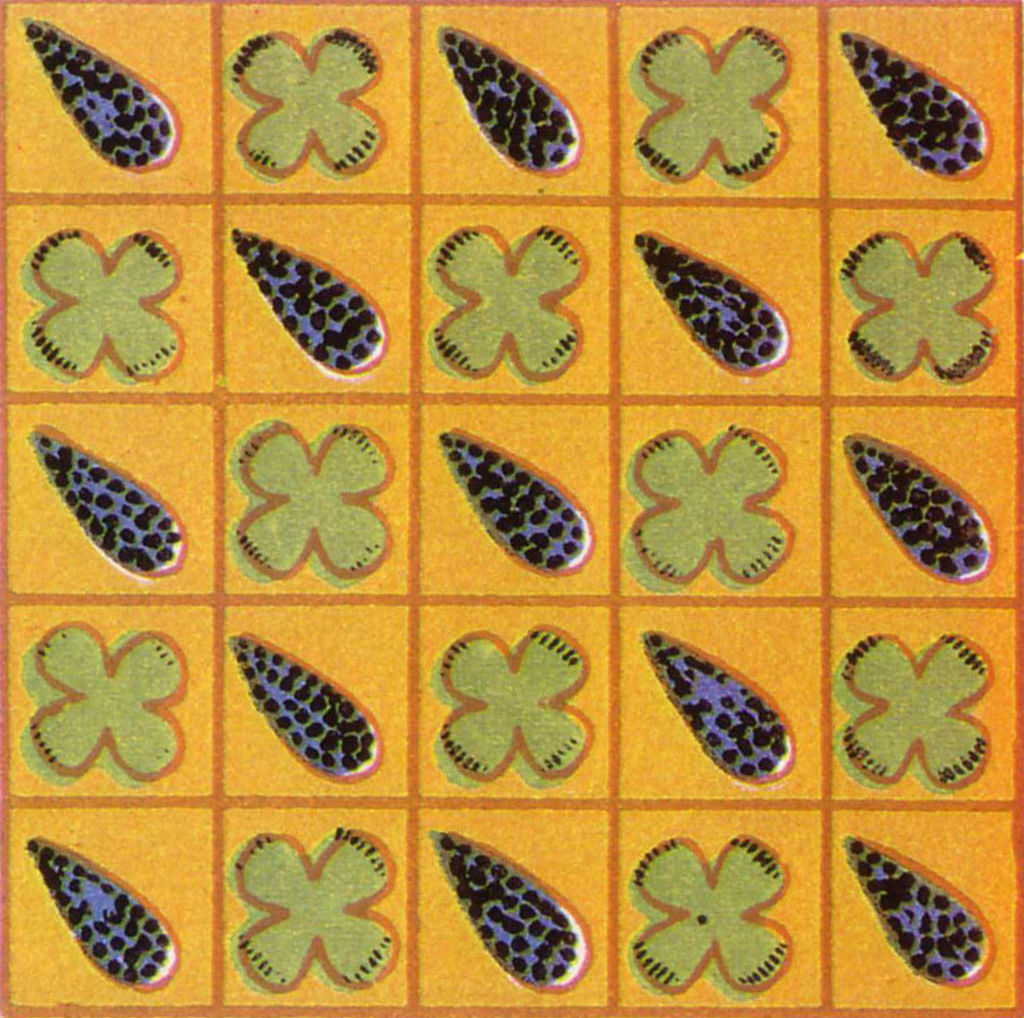
\includegraphics[width=\textwidth]{images/reflection_symmetry_wallpaper.jpg}
%        \caption{Reflectional Symmetry}
%        \label{fig:ref_sym}
%        \end{subfigure}
%        \begin{subfigure}{0.2\textwidth}
%            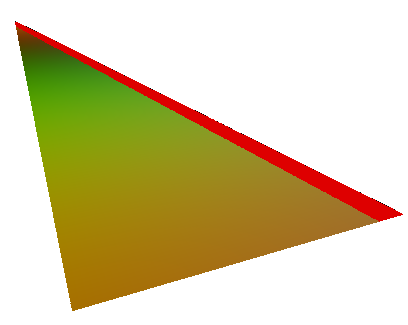
\includegraphics[width=\textwidth]{images/mirror_edge.png}
%            \caption{Mirror Edge}
%            \label{fig:me}
%        \end{subfigure}
%        \caption{Folding Symmetries}
%        \label{fig:sym}
%    \end{figure}
%
%\begin{figure}
%\centering
%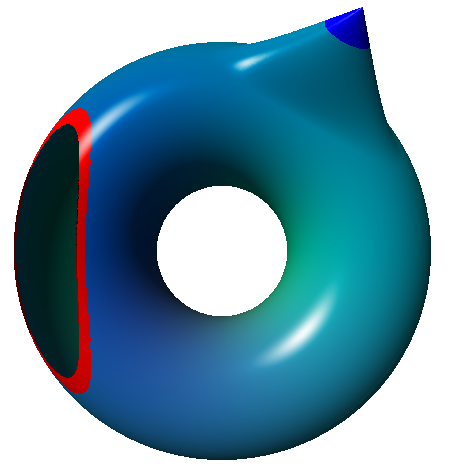
\includegraphics[width=0.3\textwidth]{images/orbifold_ex.png}
%\caption{Orbifold Visualization}
%\label{fig:orb}
%\end{figure}



\begin{definition}[Laplace spectra]
We now define the notion of \emph{Laplace spectra}. First, we define the
\emph{Laplacian Operator} $\Delta$ such that $\Delta f \coloneqq
-\grad(\divergence(f))$ for some function $f$. Then, for some orbifold
$\mathcal{O}$ we consider the function $\psi$ defined over all
$\mathbf{x} \in \mathcal{O}$. Then, consider the eigenvalue equation
$\Delta \psi(\mathbf{x}) =  -\lambda \psi(\mathbf{x})$. Applying
appropriate boundary conditions gives rise to a discrete unbounded list of
real eigenvalue solutions $0 \geq \lambda_1 \geq \lambda_2 \geq \lambda_3
\dots$. We call this resulting sequence $\{\lambda_i\}$ the \emph{Laplace
spectrum}.
\end{definition}

\section{Research Question}
We can now state our research question precisely as: given the Laplace
Spectrum of some orbifold $\mathcal{O}$, what properties can we deduce about
$\mathcal{O}$? Or equivalently: what orbifolds can we guarantee will have
different Laplace spectra?

Laplace spectra are a mathematical formalization of resonance
frequencies, so an intuitive interpretation of the question is: what
properties can we ``hear'' in an orbifold? Mark Kac popularized this type
of question in the article `Can one hear the shape of a drum?'\cite{Kac}.

\section{Result}

We present a definition in preparation for our resulting theorem.

\begin{definition}[Local Orientability]

For some chart in an orbifold $\mathcal{O}$, we take the corresponding
subset $\widetilde{U} \subset \mathcal{O}$ and topological quotient with
respect to group $\Gamma$. Then, we say that $\widetilde{U}$ is
\emph{orientable} if all elements $\Gamma$ are orientation-preserving
isometries. An orbifold $\mathcal{O}$ is \emph{locally orientable} if
every chart on $\mathcal{O}$ is orientable.  Conversely, an orbifold
$\mathcal{O}$ is \emph{locally non-orientable} if there exists a single
chart on $\mathcal{O}$ that is not orientable.
\end{definition}

Now, we present the result of our research.

\begin{theorem*}
    A locally orientable orbifold and a locally non-orientable orbifold
    will have a different Laplace spectra. Or, you can hear the local
    orientability of an orbifold.
\end{theorem*}

Simply put, we proved that orbifolds with a group containing
orientation-reversing operations will always have a different Laplace
spectra than orbifolds that have no such group.

This theorem is a generalization of Theorem 5.1 from `Asymptotic
Expansion'\cite{DGGW}. Theorem 5.1 concludes a manifold and an orbifold
with specific strata have different Laplace spectra. This Theorem 5.1
follows from our slightly stronger local orientability theorem.
Additionally, we use the concept of local orientability to present the
theorem, which is a simpler formulation of the result.

%\begin{figure}[h]
%    \centering
%        \begin{subfigure}{0.25\textwidth}
%            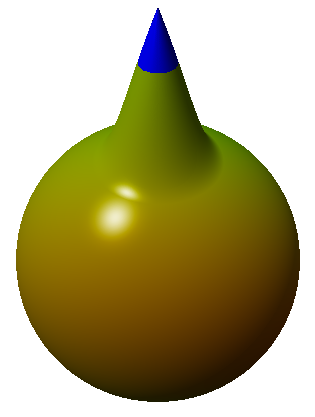
\includegraphics[width=\textwidth]{images/teardrop.png} 
%        \end{subfigure}
%        \begin{subfigure}{0.25\textwidth}
%            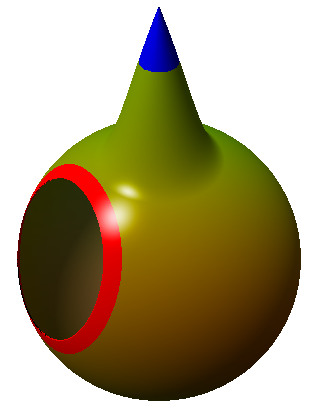
\includegraphics[width=\textwidth]{images/teardrop_edge.png}
%        \end{subfigure}
%        \caption{Non-isospectral Orbifolds}
%        \label{fig:result_ex}
%\end{figure}

\section{Asymptotic Heat Expansion}
To approach this problem, we use the asymptotic heat expansion technique as
discussed in `Asymptotic Expansion Orbifolds'\cite{DGGW}. In approximating
how heat moves through the orbifold, we obtain
a series of the form $H(t) = \sum_{k=-\dim(\orb)}^{\infty} h_{k/2}
t^{k/2}$. Every orbifold has a such a series. 
Importantly, `Asymptotic Expansion' demonstrates that two orbifolds
have the same Laplace spectra exactly when the orbifolds have the same heat
expansion.

In combining 4.5, 4.7, and 4.8 in `Asymptotic Expansion' we have
that an orbifold $\orb$ with collection of strata $S(\orb)$ has the
following heat expansion:

\begin{equation}
    H(t) = {(4\pi t)}^{-\dim(\mathcal{O})/2}\sum_{k=0}^{\infty}a_k(\mathcal{O})t^k
            +\sum_{N \in S(\mathcal{O})}\frac{{(4\pi t)}^{-\dim(N)/2}}{\myabs{\iso(N)}}\sum_{k=0}^{\infty}t^k\int_{N} \sum_{\gamma \in \iso^{\max}(\widetilde{N})}b_k(\gamma,x) dvol_N
            \label{eq:H(t)}
\end{equation}

There are a few important take-aways from this formula. 
Without loss of generality, we study odd dimensional orbifolds.
Firstly, the strata in the orbifold affect the expansion.  Importantly, for
an odd dimension orbifold, the only way for an expansion to have a non-zero
$t^{k}$ term where $k$ is some integer is by containing some \emph{even
dimensional strata}. This fact is essential in proving the result.

\section{Proof}

The proof of this theorem is a strong representation of what I specifically
contributed to the project. My research mentor Liz Stanhope and I worked
together on this theorem in the dimension $3$ case. Then, I conjectured
that the theorem holds in the $n$ dimensional case and presented a rough
proof. My research mentor pointed out various gaps in the proof that we
filled in together, resulting in a finished proof. Below I present a
simplified version of this proof which is the primary achievement of the
research.

\begin{proof}

Take $\mathcal{O}_o$ to be a locally orientable orbifold and
$\mathcal{O}_n$ to be a locally non-orientable orbifold. Then, we claim
that $\mathcal{O}_o$ and $\mathcal{O}_n$ have different Laplace spectra. 

It is known that orbifolds of different dimensions have different Laplace
spectra, thus we conclude $\dim(\orb_o) =
\dim(\orb_n)$. Without loss of generality, we take this dimension to be
odd.

We first claim that every integer power coefficient in the heat expansion of
$\mathcal{O}_o$ is $0$. We proceed by the method of contradiction under the
assumption there exists some non-zero coefficient.  Then, as noted
previously, it follows from Equation~\ref{eq:H(t)} that $\orb_o$ has some
even dimensional primary strata $N$. As discussed in the definition, the nature of
primary strata implies there exists some isometry $\gamma \in \iso(N)$ such
that $\dim(\fix(\iso(N))) = \dim(N)$. But, because $N$ is even and
$\dim(\orb)$ is odd, this implies that $\gamma$ is orientation reversing,
which contradicts the locally orientable nature of $\orb$. Thus, every
integer power coefficient in the heat expansion is $0$, verifying the
claim.

We next claim that at least one integer power coefficient in $\orb_n$ is
non-zero. Firstly, $\orb_n$ must have at least one non-orientable chart
$(\widetilde{U}, \Gamma, \pi_U)$ by the construction of $\orb_n$. So, there
is some orientation-reversing operation $\gamma \in \Gamma$. Because
$\orb_n$ is odd, it follows that $\fix(\gamma)$ is even. With a small
argument, it follows from $2.14$ in \cite{DGGW} that there exists at least one primary
strata of the dimension of $\fix(\gamma)$, which is even.
Then, we consider the strata of the maximal dimension $n$. It follows from
Equation~\ref{eq:H(t)} that only strata of maximal dimension affect the
$-n/2$ term in the expansion. Furthermore, the $-n/2$ term contributed by
each strata of maximal dimension strictly positive. Thus the final $-n/2$
is simply a sum of positive values and thus is strictly greater than $0$.
Note that $n$ is even, so we have a non-zero integer power coefficient in
$\orb_n$, verifying the claim.

Thus, we know that there exists at least one term in the heat expansion of
$\orb_o$ and $\orb_n$ that differ. Thus, as discussed above, the two
orbifolds have different Laplace spectra, concluding the proof of this
theorem.
%\begin{figure}[h]
%\centering
%\begin{tabular}{c | c c c c c c c}
%    & \dots & $t^{-1}$ & $t^{-1/2}$ & $t^{0}$ & $t^{1/2}$ & $t^{1}$ & \dots\\
%\hline
%$\mathcal{O}_o$ &
%    \dots & $0$ & $\#$ & $0$ & $\# $& $0$ & \dots \\
%$\mathcal{O}_n$ &
%\dots & $d_{-1}$ & $\#$ & $d_0$ & $\# $& $d_1$ & \dots  \\
%\end{tabular}
%\caption{Heat expansion coefficients}
%\end{figure}
\end{proof}

\section{Future Work}

We have looked into applying the asymptotic heat expansion machinery to the
specific class of three dimensional flat orbifolds. Conway names this class
of orbifolds \emph{platycosms}\cite{platy} and provides a complete listing of
the corresponding crystallographic space group in the book \textit{The
Symmetries of Things}\cite{SOT}. In finding heat expansion coefficients of
various platycosms, we could potentially conclude that some platycosms have
different Laplace spectra. This would involve classifying all primary
strata in each of the $230$ different platycosms, which are necessary to
compute heat expansion terms. It appears that it is possible to automate
this process with computing.

\bibliographystyle{plain}
\nocite{*}
\bibliography{references}

\end{document}
